\section{Algebralliset käyrät ja projektiiviset avaruudet}
Tämän osion tarkoituksena on esitellä tiiviisti algebrallisten käyrien, projektiivisten avaruuksien ja projektiivisten käyrien määritelmän sanaston kiinnittämiseksi. Kiinnostunut lukija löytää huolellisemman tarkastelun esimerkiksi Gathmannin algebrallisen geometrian luentomuistiinpanoista \citep{gathmann-ag}.

\subsection{Affiinit algebralliset käyrät kompleksitasossa}
Affiini algebrallinen käyrä kompleksitasossa on määritelty polynomin nollakohtien joukkona. Algebrallinen käyrä eroaa polynomista siten, että algebrallinen käyrä on jonkin polynomin nollakohtajoukko. 
\begin{maaritelma}
    Jos $f\in\C[x,y]$ on ei-vakio polynomi, niin sen affiini algebrallinen käyrä $C$ on
    \begin{equation*}
        C = \{ (x,y) \in \mathbb{C}^2 \mid f(x,y) = 0 \}.
    \end{equation*}
\end{maaritelma}
Yleisesti $n$-ulotteinen algebrallinen hyperpinta on $n+1$-ulotteisen polynomin nollakohtajoukko. Kuvassa~\ref{kuva:algebrallinen-käyrä} havainnollistetaan tätä 2-pinnalla ja sen $xy$-tasoon jättämällä ellipsillä.
\begin{figure*}
    \centering
    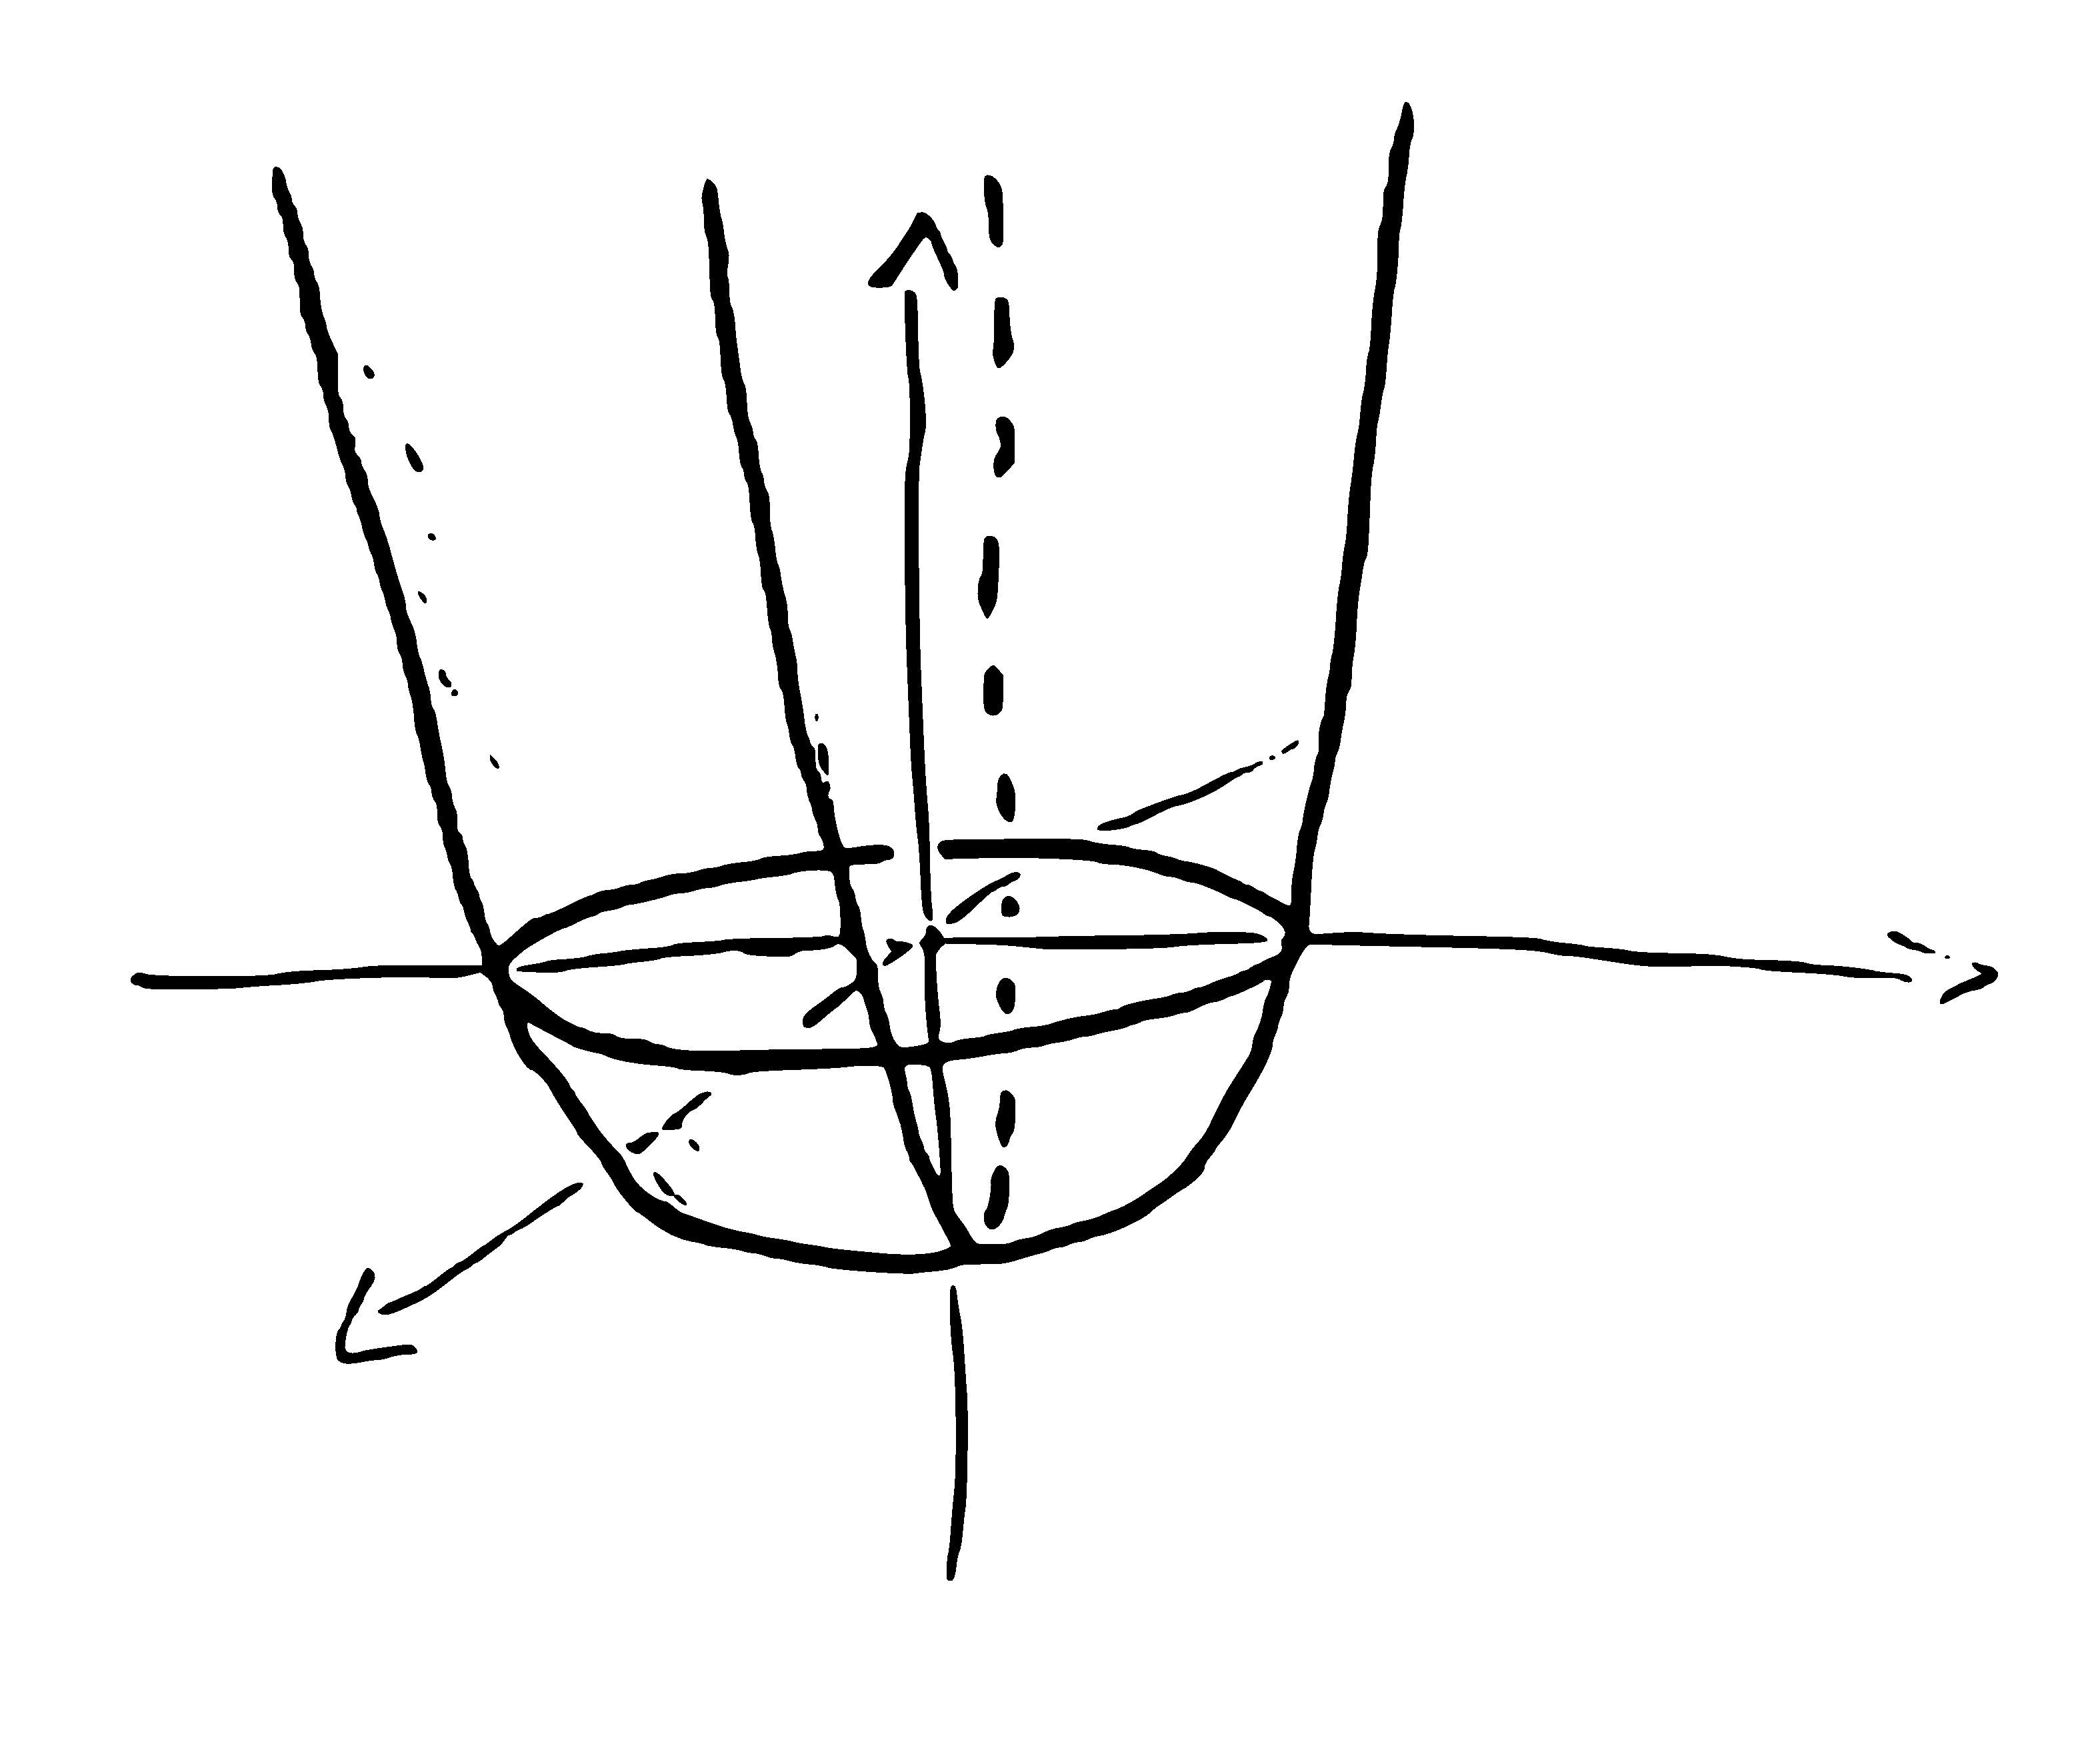
\includegraphics[width=0.5\textwidth]{figures/algebrallinen-käyrä.pdf}
    \caption{Parabolinen pinta $f(x,y)-z=0$ ja algebrallinen käyrä $f(x,y)=0$.}
    \label{kuva:algebrallinen-käyrä}
\end{figure*}
\begin{maaritelma}
    Olkoon $S\subset\K[x_1,\dots,x_n]$ joukko polynomeja. $S$:n \emph{(affiini) varisto} on
    \begin{align*}
        V(S):=\{x\in\K^n:f(x)=0\text{ kaikille }f\in S\}.
    \end{align*}
    Vastaavasti jos $X\subset\K^n$ on mikä tahansa joukko, 
    \begin{align*}
        I(X):=\{f\in\K[x_1,\dots,x_n]:f(x)=0\text{ kaikille }x\in X\}
    \end{align*}
    on $X$:n \emph{ideaali}.
\end{maaritelma}
Tästä lähtien polynomia $f$ vastaavaa käyrää voidaan merkitä vain $V(f)$.
\begin{maaritelma}
    Olkoon $V(f)$, $f\in\C[x,y]$ algebrallinen käyrä. Kirjoitetaan
    \begin{equation*}
        f(x,y)=\sum_{i,j=0}^{N}a_{ij}x^iy^j,\quad N\in\N,a_{ij}\in\C.
    \end{equation*}
    Tällöin $V(f)$:n tai $f$:n aste on $\deg(V(f))=\deg(f)=\max\{i+j\}$.
\end{maaritelma}
Varistot ja ideaalit tarjoavat tärkeän yhteyden käyrien tai pintojen geometrian ja abstraktin algebran välillä. Eräs tärkeä huomio koskee variston käyttäytymistä yhdisteiden suhteen. Olkoot $S,T\subset\K[x_1,\dots,x_n]$ kaksi kokoelmaa polynomeja. Tällöin $x\in V(S)\cup V(T)$ kuuluu molempien polynomijoukkojen piirtämään hyperpintaan täsmälleen silloin, kun $x$ on $S$:n ja $T$:n polynomien nollakohta. Toisin sanoen
\begin{align*}
    V(S)\cup V(T)=V(S\cap T).
\end{align*}
Jos $S=\{f\}$ ja $T=\{g\}$, niin ehto muuntuu muotoon
\begin{align*}
    V(f)\cup V(g)=V(\{f\}\cap\{g\})=V(fg),
\end{align*}
missä $fg$ on vain polynomien tulo. Erityisen hyödyllistä tämä voi olla polynomin pelkistymättömyyden hahmottamisessa.
\begin{maaritelma}
    Olkoon $f\in\K[x_1,\dots,x_n]$. Polynomi $f$ on pelkistymätön, jos kaikille $g,h\in\K[x_1,\dots,x_n]$ siten, että $f=gh$ pätee $g\in\K$ tai $h\in\K$.
\end{maaritelma}
Polynomi on siis pelkistymätön jos sitä ei voi kirjoittaa kahden epävakion polynomin tulona, tai jos sen varistoa ei voi kirjoittaa kahden variston yhdisteenä!

Eräs myöhemmin hyödyllinen erityistapaus on $n$-pallo $\S^n$.
\begin{align*}
    \S^n&=\{(x_1,\dots,x_n)\in\K^n:x_1^2+\cdots+x_n^2=1\} \\
    &=V(x_1^2+\cdots+x_n^2-1)
\end{align*}
Intuitiivisesti lienee selvää, että tapauksessa $n=0$ pallo $\S^0$ pelkistyy, mutta tapauksissa $n=1,2$ pallon ei pitäisi pelkistyä, koska ympyrää tai pallopintaa ei voi hajoittaa pienempiin osiin. Tämä on mahdollista todistaa kaikille $n>0$.
\begin{lemma}
    \label{lemma:pallo-on-pelkistymätön}
    Olkoon $n>0$ kokonaisluku. Tällöin $n$-pallon $\S^n$ määrittelevä polynomi
    \begin{align*}
        s_n(x)=x_1^2+\cdots+x_n^2-1
    \end{align*}
    on pelkistymätön.
\end{lemma}
\begin{proof}
    Polynomin $s_n$ aste on $\deg s_n=2$. Oletetaan, että $s_n$ on pelkistyvä. Tällöin on olemassa kaksi polynomia $f,g\in\K[x_1,\dots,x_n]$ siten, että $s_n=fg$ ja $f,g$ eivät kumpikaan ole vakioita.

    Tutkimalla asteita huomataan, että 
    \begin{align*}
        \deg s_n&=\deg f+\deg g \\
        2&=\deg f+\deg g.
    \end{align*}
    Koska $\deg f,\deg g>0$ niin $\deg f=\deg g=1$. Siis $f$ ja $g$ ovat hypertasoja, muotoa $c_0+c_1x_1+\cdots+c_nx_n=0$. Tällöin
    \begin{align*}
        \S^n=V(s_n)=V(f)\cup V(g)
    \end{align*}
    on kahden hypertason yhdiste. Intuitiivisesti ottaen tämä on mahdotonta, sillä $n$-pallolla on $n$-ulotteista kaarevuutta jokaisessa pisteessä, mutta hypertaso on $n$-ulotteisesti litteä jokaisessa pisteessä. 

    Täsmällisesti tämä voidaan muotoilla normaalivektorin avulla. Litteän pinnan normaalivektori on pisteestä riippumatta saman suuntainen, kun taas kaarevan pinnan normaalivektori riippuu pisteestä. Normaali voidaan laskea gradientin avulla. Kirjoitetaan
    \begin{align*}
        f(x_1,\dots,x_n)=\sum_{i=0}^{n}a_ix_i^2,\qquad
        g(x_1,\dots,x_n)=\sum_{i=0}^{n}b_ix_i^2.
    \end{align*}
    Tällöin normaalit ovat
    \begin{align*}
        \vec n_{s_n}&:\nabla s_n=\left[2x_1,\dots,2x_n\right]^T \\
        \vec n_f&:\nabla f=\left[a_1,\dots,a_n\right]^T \\
        \vec n_g&:\nabla g=\left[b_1,\dots,b_n\right]^T.
    \end{align*}
    ja selvästi on olemassa $(x_1,\dots,x_n)\in\K^n$ siten, että 
    \begin{align*}
        \vec n_{s_n}(x_1,\dots,x_n)&\ne\vec f(x_1,\dots,x_n),\quad\text{ja} \\
        \vec n_{s_n}(x_1,\dots,x_n)&\ne\vec g(x_1,\dots,x_n).
    \end{align*}
    Siispä $s_n=fg$ on ristiriita, joten $s_n$ on pelkistymätön.
\end{proof}


\subsection{Singulariteetit ja säännöllisyys}
Käyrän $V(f)$ paikallinen muoto pisteessä $p=(a,b)\in V(f)$ määrittyy $f$:n osittaisderivaattojen avulla. 
\begin{maaritelma}
    Käyrän $V(f)$ piste $p=(a,b)\in V(f)$ on \emph{singulaarinen}, jos $f$:n osittaisderivaatat häviävät pisteessä $p$:
    \begin{equation*}
        \frac{\partial f}{\partial x}(a,b) = 0 \quad \text{ja} \quad \frac{\partial f}{\partial y}(a,b) = 0.
    \end{equation*}
    Tällöin voidaan myös sanoa, että käyrä on \emph{singulaarinen}.
\end{maaritelma}
\begin{maaritelma}
    Jos vähintään yksi osittaisderivaatoista ei ole nolla $p$:ssä, niin piste on \emph{säännöllinen}. Jos kaikki käyrän pisteet ovat säännöllisiä, niin käyrä on \emph{säännöllinen}.
\end{maaritelma}
Säännöllisessä pisteessä implisiittifunktiolause takaa, että käyrä näyttää paikallisesti (kompleksimielessä, $\dim_\C$) 1-ulotteiselta monistolta\footnote{Oikea termi olisi \emph{varisto}, joka tiiviyden vuoksi jätetään määrittelemättä. Työn tarpeisiin monisto riittää hyvin.}, ja on mahdollista määritellä yksikäsitteinen tangenttisuora. Kuvassa~\ref{kuva:käyriä-ja-singulariteetteja} on havainnollistettu singulaarisuutta. Singulaarinen käyrä voi leikata itseään tai muodostaa kärjen. Koska polynomit ovat kaikissa pisteissään derivoituvia, on singulaarisen käyrän kokonaisderivaatan oltavat huonosti käyttäytyvässä pisteessä nolla.
\begin{figure*}
    \centering
    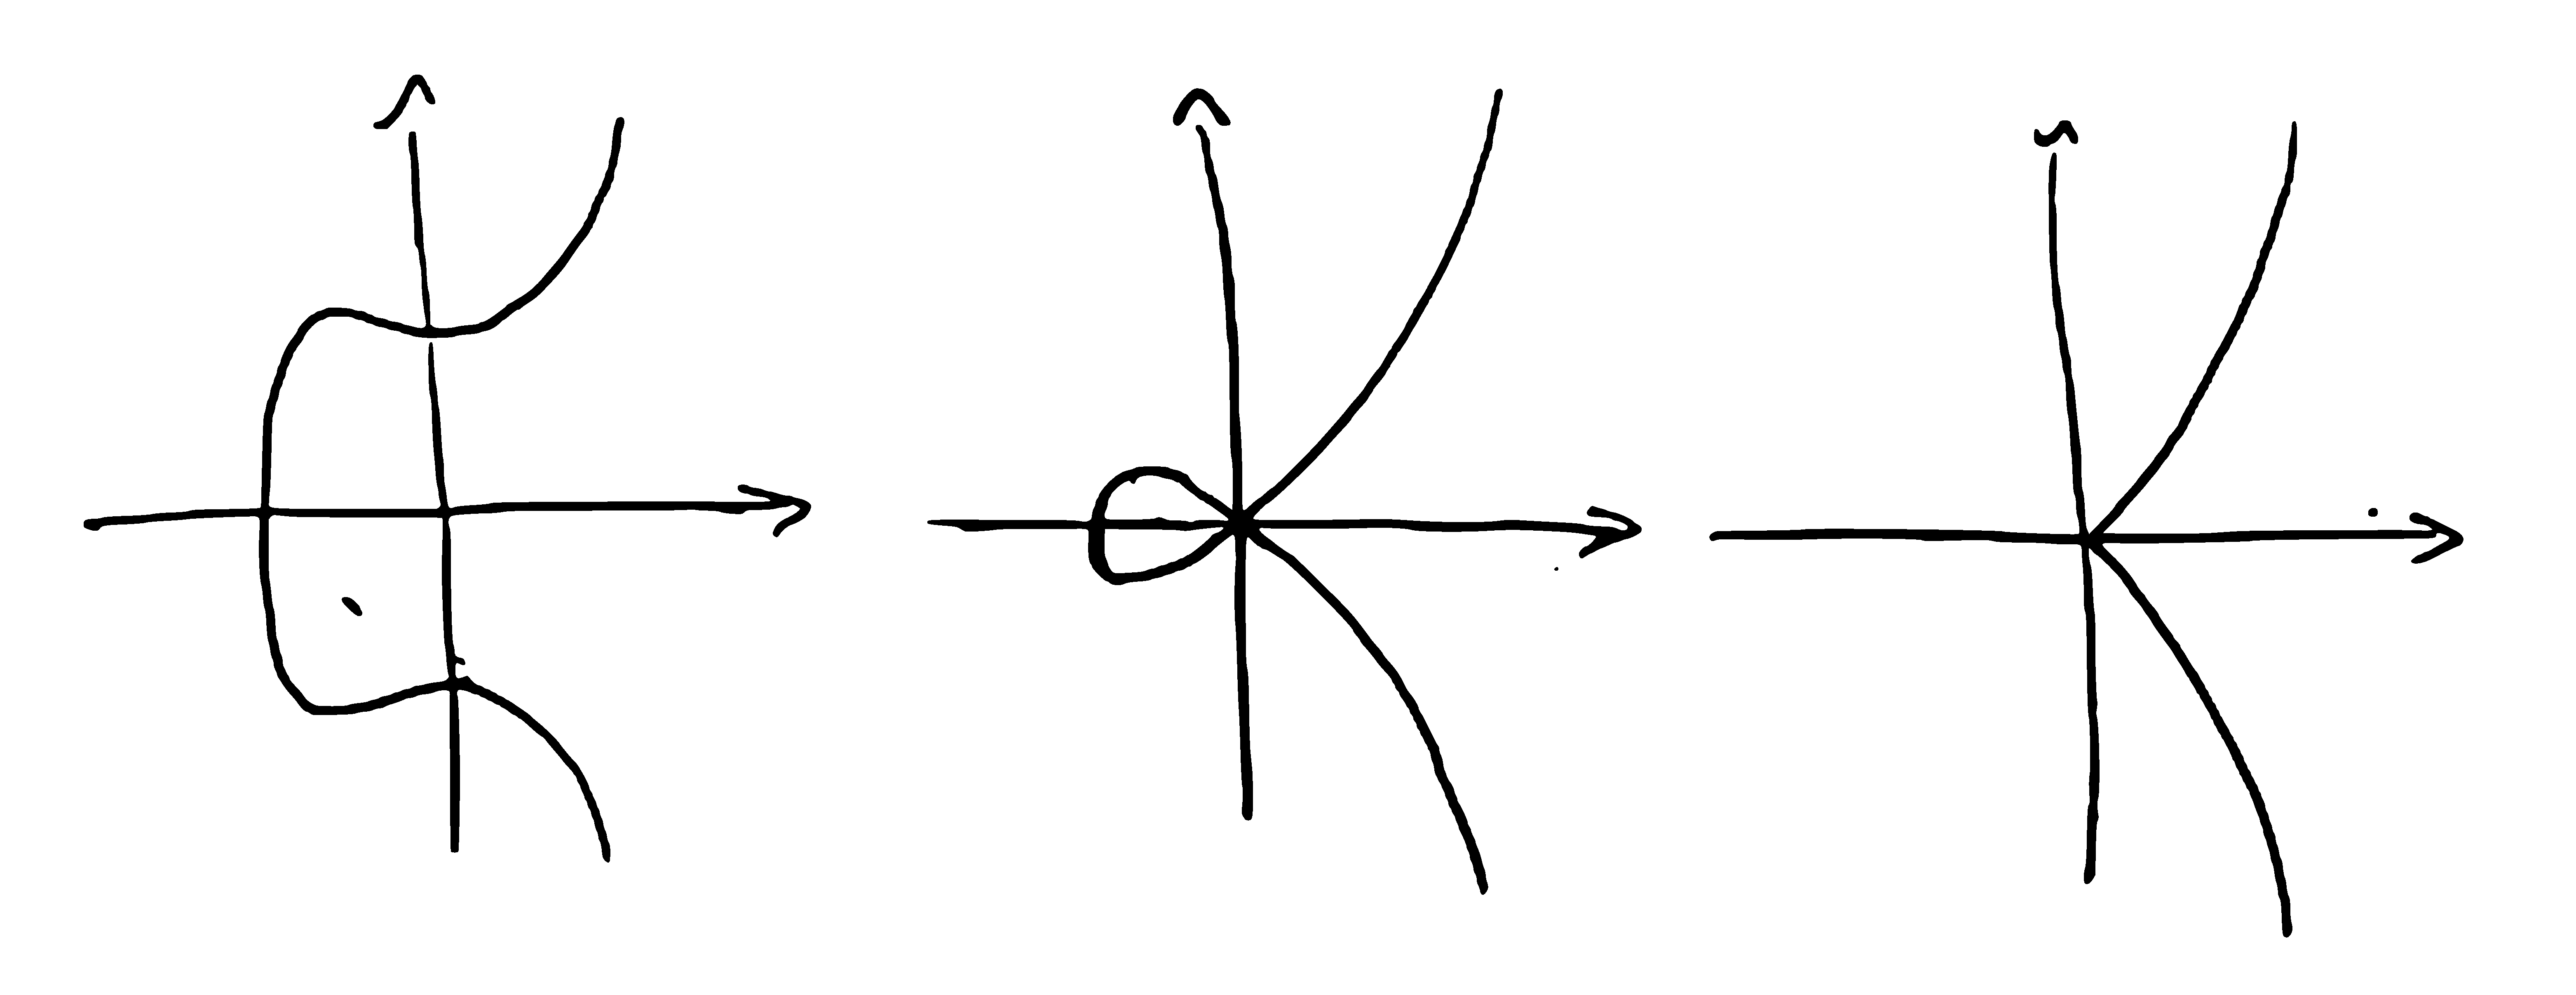
\includegraphics[width=0.7\textwidth]{figures/käyriä-ja-singulariteetteja.pdf}
    \caption{Yksi epäsingulaarinen käyrä ja kaksi singulaarista. Vasemmalta oikealle käyriä määrittävät yhtälöt ovat $y^2-x^3-x^2-1=0$, $y^2-x^3-x^2=0$ ja $y^2-x^3=0$.}
    \label{kuva:käyriä-ja-singulariteetteja}
\end{figure*}

\subsection{Projektiivinen avaruus}
Avaruudella $\K^n$ on geometrinen rajoitus: kaksi erillistä suoraa leikkaavat yleensä yhdessä pisteessä, paitsi jos ne ovat yhdensuuntaisia. Käsitteiden yhtenäistämiseksi käyttöön otetaan projektiivinen avaruus, joka lisää tavalliseen vektoriavaruuteen $\K^n$ matemaattisesti hyvin määritellyn ``horisontin''.

$\K$-rakenteinen $n$-ulotteinen projektiivinen avaruus $\P^n(\K)$ määritellään joukoksi, joka koostuu avaruuden $\K^{n+1}$ vektorisäteistä (eli niiden ekvivalenssiluokista), jotka kulkevat origon kautta.
\begin{maaritelma}
    Olkoon $(Z_0,\dots,Z_n) \in \K^{n+1}-\{0\}$. Määritellään ekvivalenssirelaatio $\sim$ seuraavasti:
    \begin{equation*}
        (Z_0,\dots,Z_n) \sim (\lambda Z_0, \dots, \lambda Z_n) \quad \text{kaikille } \lambda \in \K^*.
    \end{equation*}
    Tällöin
    \begin{equation*}
        \P^n(\K):=\frac{\K^{n+1}-\{0\}}{\sim}.
    \end{equation*}
    Ekvivalenssiluokan edustaja merkitään homogeenisilla koordinaateilla $[Z_0:\dots:Z_n]$.
\end{maaritelma}
\begin{asetus}
    Jatkossa tarkastellaan yksinomaan kompleksista projektiivista avaruutta $\P^n(\C)$. Lisäksi merkitään $\P^n$ pidemmän $\P^n(\C)$ sijasta.

    Poikkeus tehdään havainnollistavien kuvien kohdalla, jotka piirretään reaaliseen tasoon. Kompleksitasossa on liikaa ulottuvuuksia.
\end{asetus}
Projektiivisen avaruuden idea on tuoda tavalliseen avaruuteen $\K^n$ myös ``horisontti'', joka ajaa äärettömyyden virkaa. Kuvassa~\ref{kuva:projektiivinen-suora} on piirretty kaksi yhdensuuntaista suoraa tavalliseen $\R$-tasoon sekä projektiiviseen tasoon $\P^2(\R)$. Äärettömyys ei ole yksi piste, vaan kokonainen ``horisonttiviiva'' ja suorat leikkaavat suoraan katsojan edessä.
\begin{figure*}
    \centering
    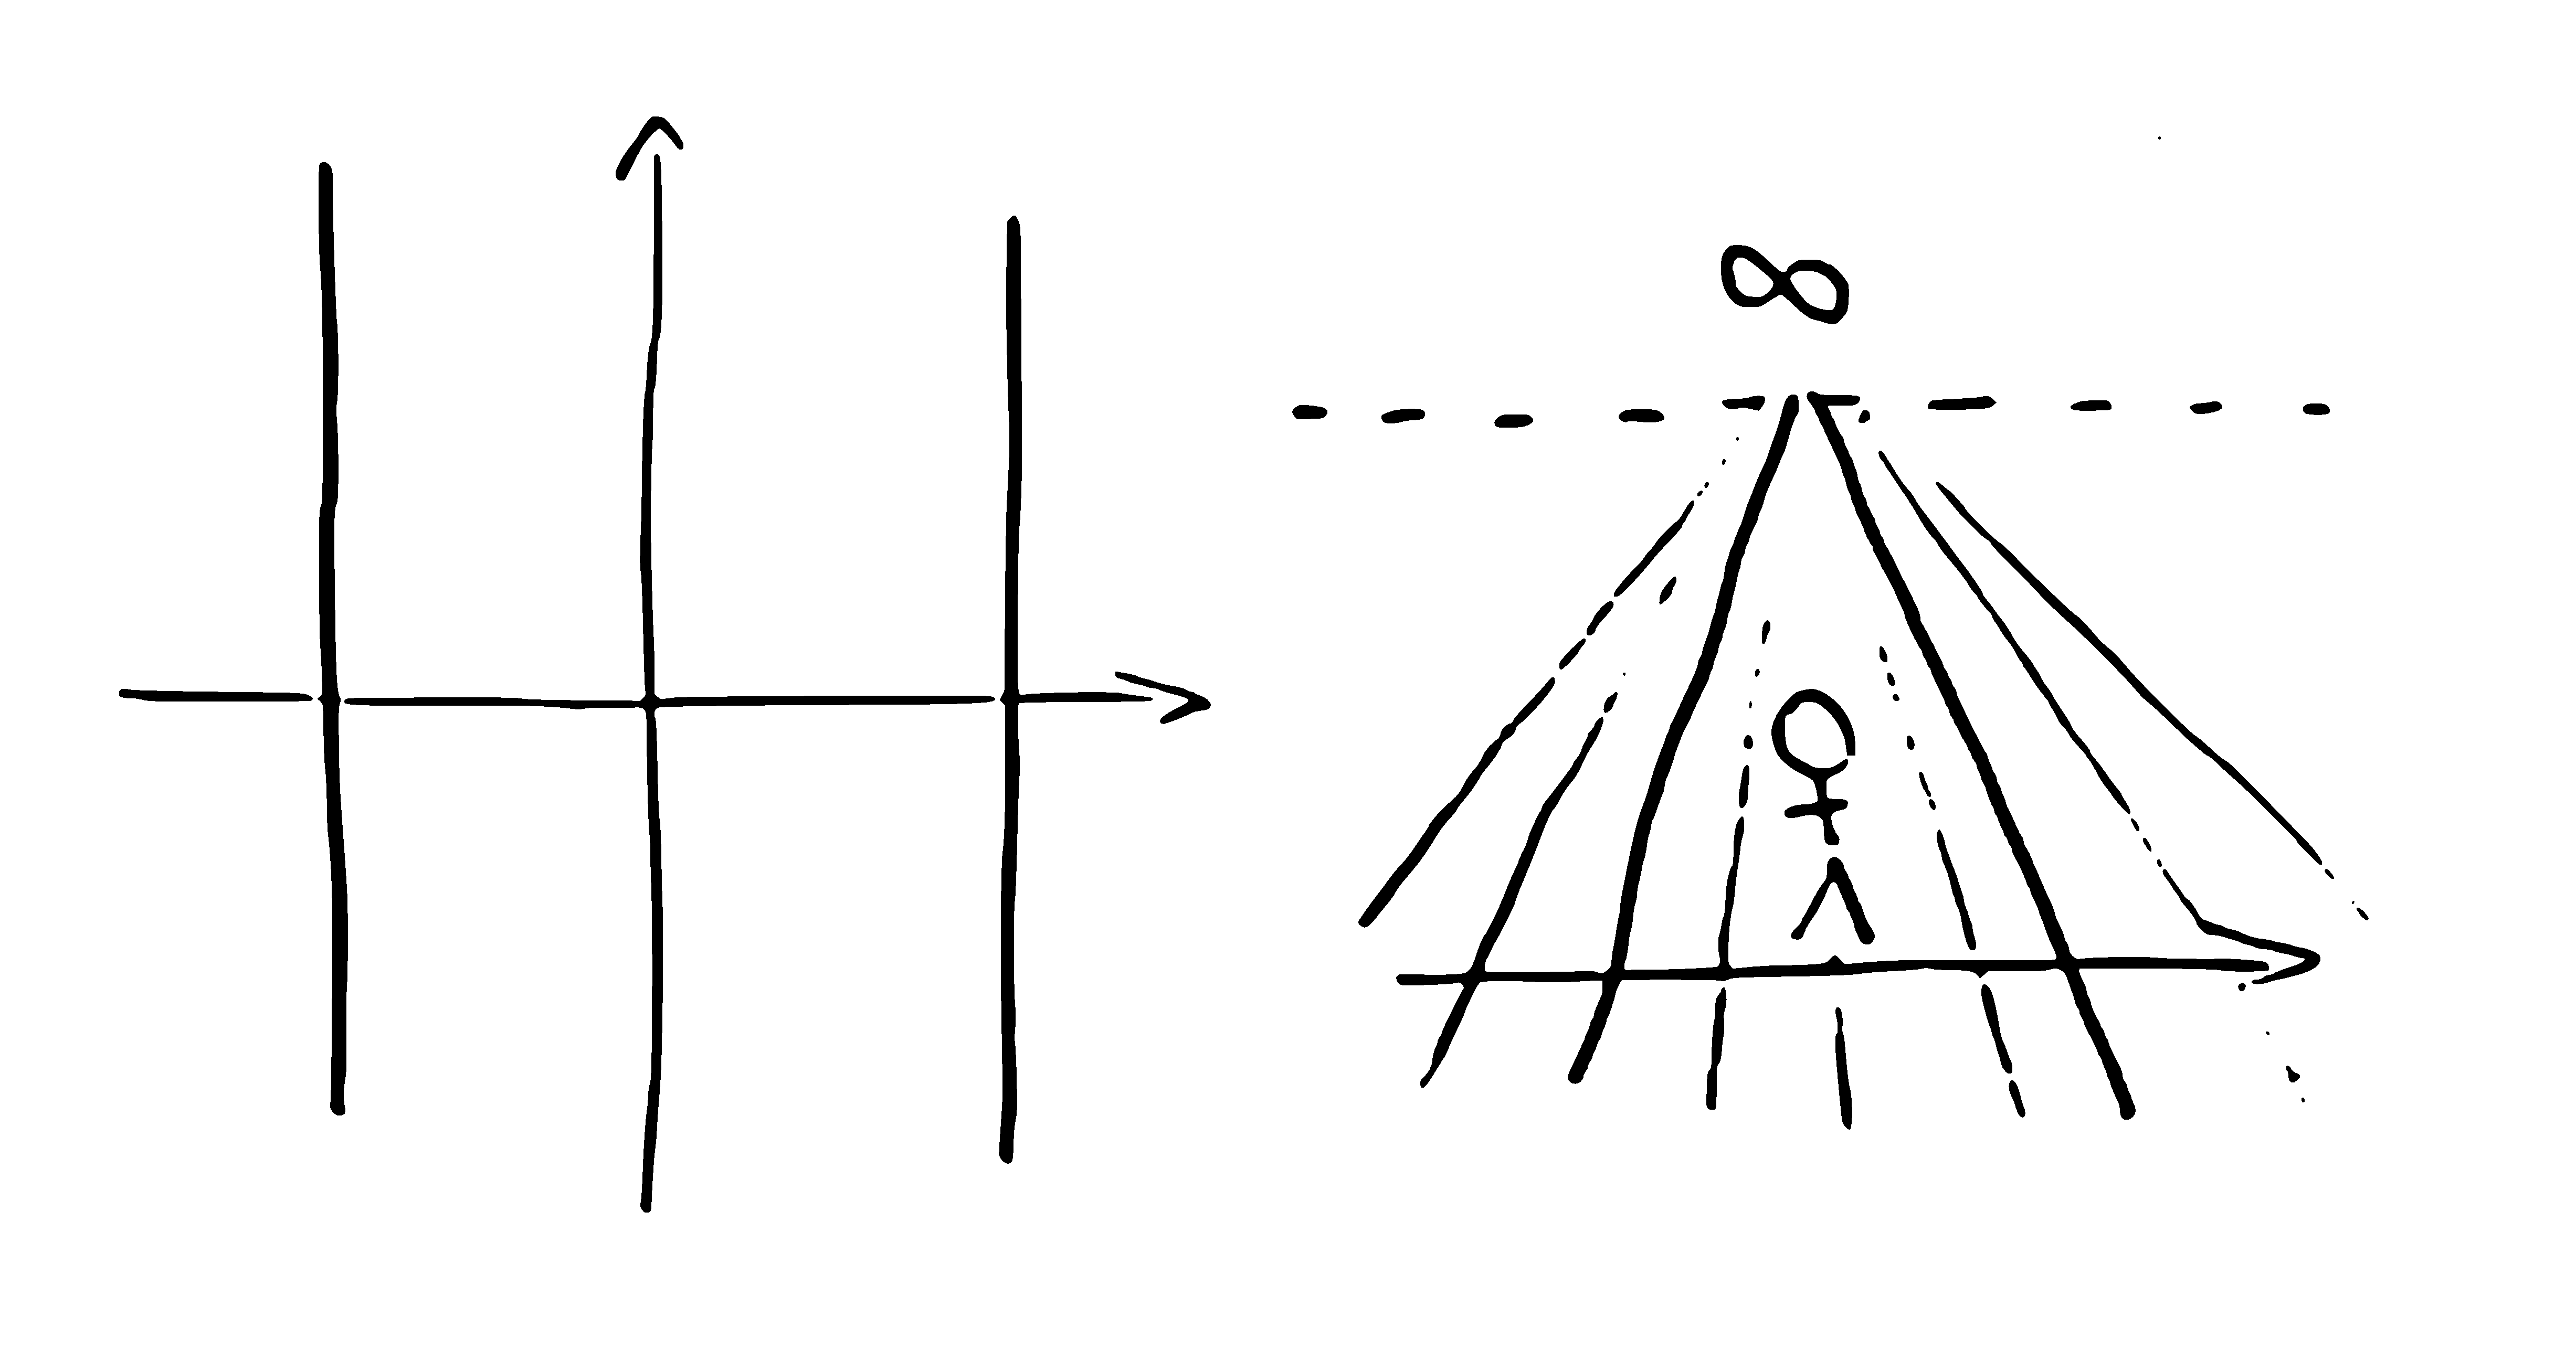
\includegraphics[width=0.7\textwidth]{figures/projektiivinen-suora.pdf}
    \caption{Projektiivisessa tasossa kaksi yhdensuuntaista suoraa leikkaavat äärettömyydessä.}
    \label{kuva:projektiivinen-suora}
\end{figure*}
Havaintoa siitä, että projektiivisessa tasossa äärettömyys on tasoa ympäröivä horisontti, tarkastellaan täsmällisemmin seuraavassa esimerkissä ja lemmassa.
\begin{esimerkki}
    \label{esim:proj-taso-ja-suora}
    Tapauksissa $n=1$ ja $n=2$
    \begin{itemize}
        \item $\P^1\cong\C\cup\{\infty\}$ (Riemann-pallo)
        \item $\P^2\cong\C^2\cup\P^1$. $\P^2$:n koordinaatit ovat $[X:Y:Z]$, ja $\P^1$ on joukko pisteitä, joilla $Z=0$.
    \end{itemize}
    Jos tarkastellaan projektiivisten avaruuksien ulottuvuuksia reaalimielessä ($\dim_\R(\C)=2$), niin $\dim_\R(\P^1)=2$ ja $\dim_\R(\P^2)=6$ (vai 4?).
\end{esimerkki}
Esimerkin~\ref{esim:proj-taso-ja-suora} kaava yleistyy itse asiassa kaikille $n\in\N$.
\begin{lemma}
    \label{lemma:projektiivisen-avaruuden-jako}
    Projektiivinen avaruus on erillinen yhdiste $\P^{n}=\C^n\sqcup\P^{n-1}$.
\end{lemma}
\begin{proof}
    Tarkastellaan $\P^{n}$:n pistettä $[Z_0:\dots:Z_{n}]$, jolla on $n$ koordinaattia. Jos $Z_{n}\neq 0$, niin piste voidaan esittää muodossa
    \begin{equation*}
        [Z_0:\dots:Z_n] \sim \left[\frac{Z_0}{Z_n}:\dots:\frac{Z_{n-1}}{Z_n}:1\right] \in \C^n.
    \end{equation*}
    Jos taas $Z_n=0$, niin piste kuuluu $\P^{n-1}$:een. Tällöin saadaan jako $\P^{n}=\C^n\sqcup\P^{n-1}$.
\end{proof}
Yleisen projektiivisen avaruuden $\P^n$ ``sisus'' on $\C^n$ ja ``kuori äärettömyydessä'' $\P^{n-1}$, joka induktiivisesti kuortaan lukuunottamatta muistuttaa $\C^{n-1}$:tä. Tämä antaa mielekkään upotuksen $\C^n\hookrightarrow\P^n$, jossa $\C^n$ upotetaan bijektiivisesti pelkästään $\P^n$:n ``sisukseen''.

Työlle relevantissa 2-ulotteisessa tapauksessa avaruus $\C^2$ voidaan nähdä paikallisena karttana (tai tiheänä avoimena joukkona) projektiivisessa tasossa $\P^2(\C)$. Tyypillinen upotus määritellään seuraavasti:
\begin{align*}
    \iota : \C^2 &\hookrightarrow \P^2(\C) \\
    (x,y) &\mapsto [x : y : 1]
\end{align*}
Pisteet $\P^2$:ssa, jotka eivät kuulu tämän upotuksen kuvaan, ovat muotoa $[X:Y:0]$. Näiden pisteiden joukko muodostaa projektiivisen suoran $\P^1$, jota kutsutaan \emph{suoraksi äärettömyydessä} tai \emph{äärettömyyssuoraksi}. Lemman \ref{lemma:projektiivisen-avaruuden-jako} hengessä $\P^2=\C^2\sqcup\P^1$.

Edellinen upotus ei ole kaikissa tilanteissa optimaalinen tai toimiva, mutta pääidea on, että upottaminen on erittäin helppoa.

\subsection{Projektiiviset käyrät}
Projektiivisessa tasossa $\P^2$ klassinen polynomi $f(x,y)$ ei ole hyvin määritelty, koska homogeeniset koordinaatit ovat ekvivalentteja skalaarikertoimen suhteen. Tämän vuoksi on käytettävä \emph{homogeenistä} polynomia $F(X,Y,Z)$, eli polynomia, jossa kaikilla monomeilla on sama aste $d$. Yhtälö $F(\lambda X, \lambda Y, \lambda Z) = \lambda^d F(X,Y,Z) = 0$ on tällöin riippumaton valitusta edustajasta.
\begin{maaritelma}[Homogenisointi]
    Polynomi $f(x,y) \in \C[x,y]$ voidaan \emph{homogenisoida} määrittelemällä
    \begin{equation*}
        F(X,Y,Z) = Z^d f\left(\frac{X}{Z}, \frac{Y}{Z}\right),
    \end{equation*}
    missä $d$ on polynomin $f$ aste.
\end{maaritelma}
\begin{maaritelma}
    Projektiivinen algebrallinen käyrä $\mathcal{C}$ määritellään homogeenisen polynomin $F(X,Y,Z)$ nollakohtien joukkona:
    \begin{equation*}
        \mathcal{C} = \{ [X:Y:Z] \in \P^2 \mid F(X,Y,Z) = 0 \}.
    \end{equation*}
\end{maaritelma}
\begin{huomautus}
    Polynomin homogenisointi sallii luonnollisesti käyrän tarkastelun myös äärettömyyssuoralla. Projektiivinen käyrä $\mathcal{C}$ on aina suljettu ja kompakti, koska se on suljettu alijoukko projektivisessa avaruudessa $\P^2$, joka on itsessään kompakti.
\end{huomautus}
Algebrallisen käyrän homogenisointi sallii varsin mielenkiintoisia näkökulmia tuttujen käyrien tarkasteluun. Jos tasoon piirtää paraabelin $y=x^2$, käyrä hajaantuu kohti äärettömyyttä $y$-akselin molemmin puolin. Hajaantuminen on kuitenkin symmetristä $y$-akselin molemmin puolin (koska $x^2=(-x)^2$!). Toisin sanoen käyrä hajaantuu molemmissa haaroissaan \emph{asymptoottisesti samankaltaisesti} eli molemmissa haaroissaan paraabeli lähestyy käytökseltään kahta yhdensuuntaista suoraa.
\begin{esimerkki}[Projektiivinen paraabeli]
    Paraabelin yhtälö on $f(x,y)=y-x^2=0$, jonka homogenisoitu muoto on $F(X,Y,Z)=YZ-X^2=0$. Konvention mukaan horisontti vastaa pisteitä, joilla $Z=0$. Yhtälö äärettömyydessä on siis $0Y-X^2=0$, jolloin pakosti $X=0$. Koska piste $[0:0:0]$ on kielletty, niin $Y\ne0$.

    Homogeeninen paraabeli leikkaa siis äärettömyyssuoran pisteessä $[0:Y:0]\sim[0:1:0]$. Tässä pisteessä käyrän osittaisderivaatat ovat
    \begin{equation*}
        \frac{\partial F}{\partial X} = -2X,\quad
        \frac{\partial F}{\partial Y} = Z,\quad
        \frac{\partial F}{\partial Z} = Y.
    \end{equation*}
    Pisteessä $[0:1:0]$ osittaisderivaatat ovat $(0,0,1)$, joten käyrä on säännöllinen. Tangenttisuora pisteessä $[0:1:0]$ on siis $Z=0$, eli äärettömyyssuora. Tämä tarkoittaa sitä, että paraabelin molemmat haarat yhtyvät tangentiaalisesti äärettömyydessä.
\end{esimerkki}

Koska projektiivisessa avaruudessa pisteet ovat suorien ekvivalenssiluokkia, tarkoittaa asymptoottinen samankaltaisuus hajaantumisessa sitä, että haarat yhtyvät horisontissa. Tämä on piirretty kuvaan~\ref{kuva:projektiivinen-paraabeli}.
\begin{figure*}
    \centering
    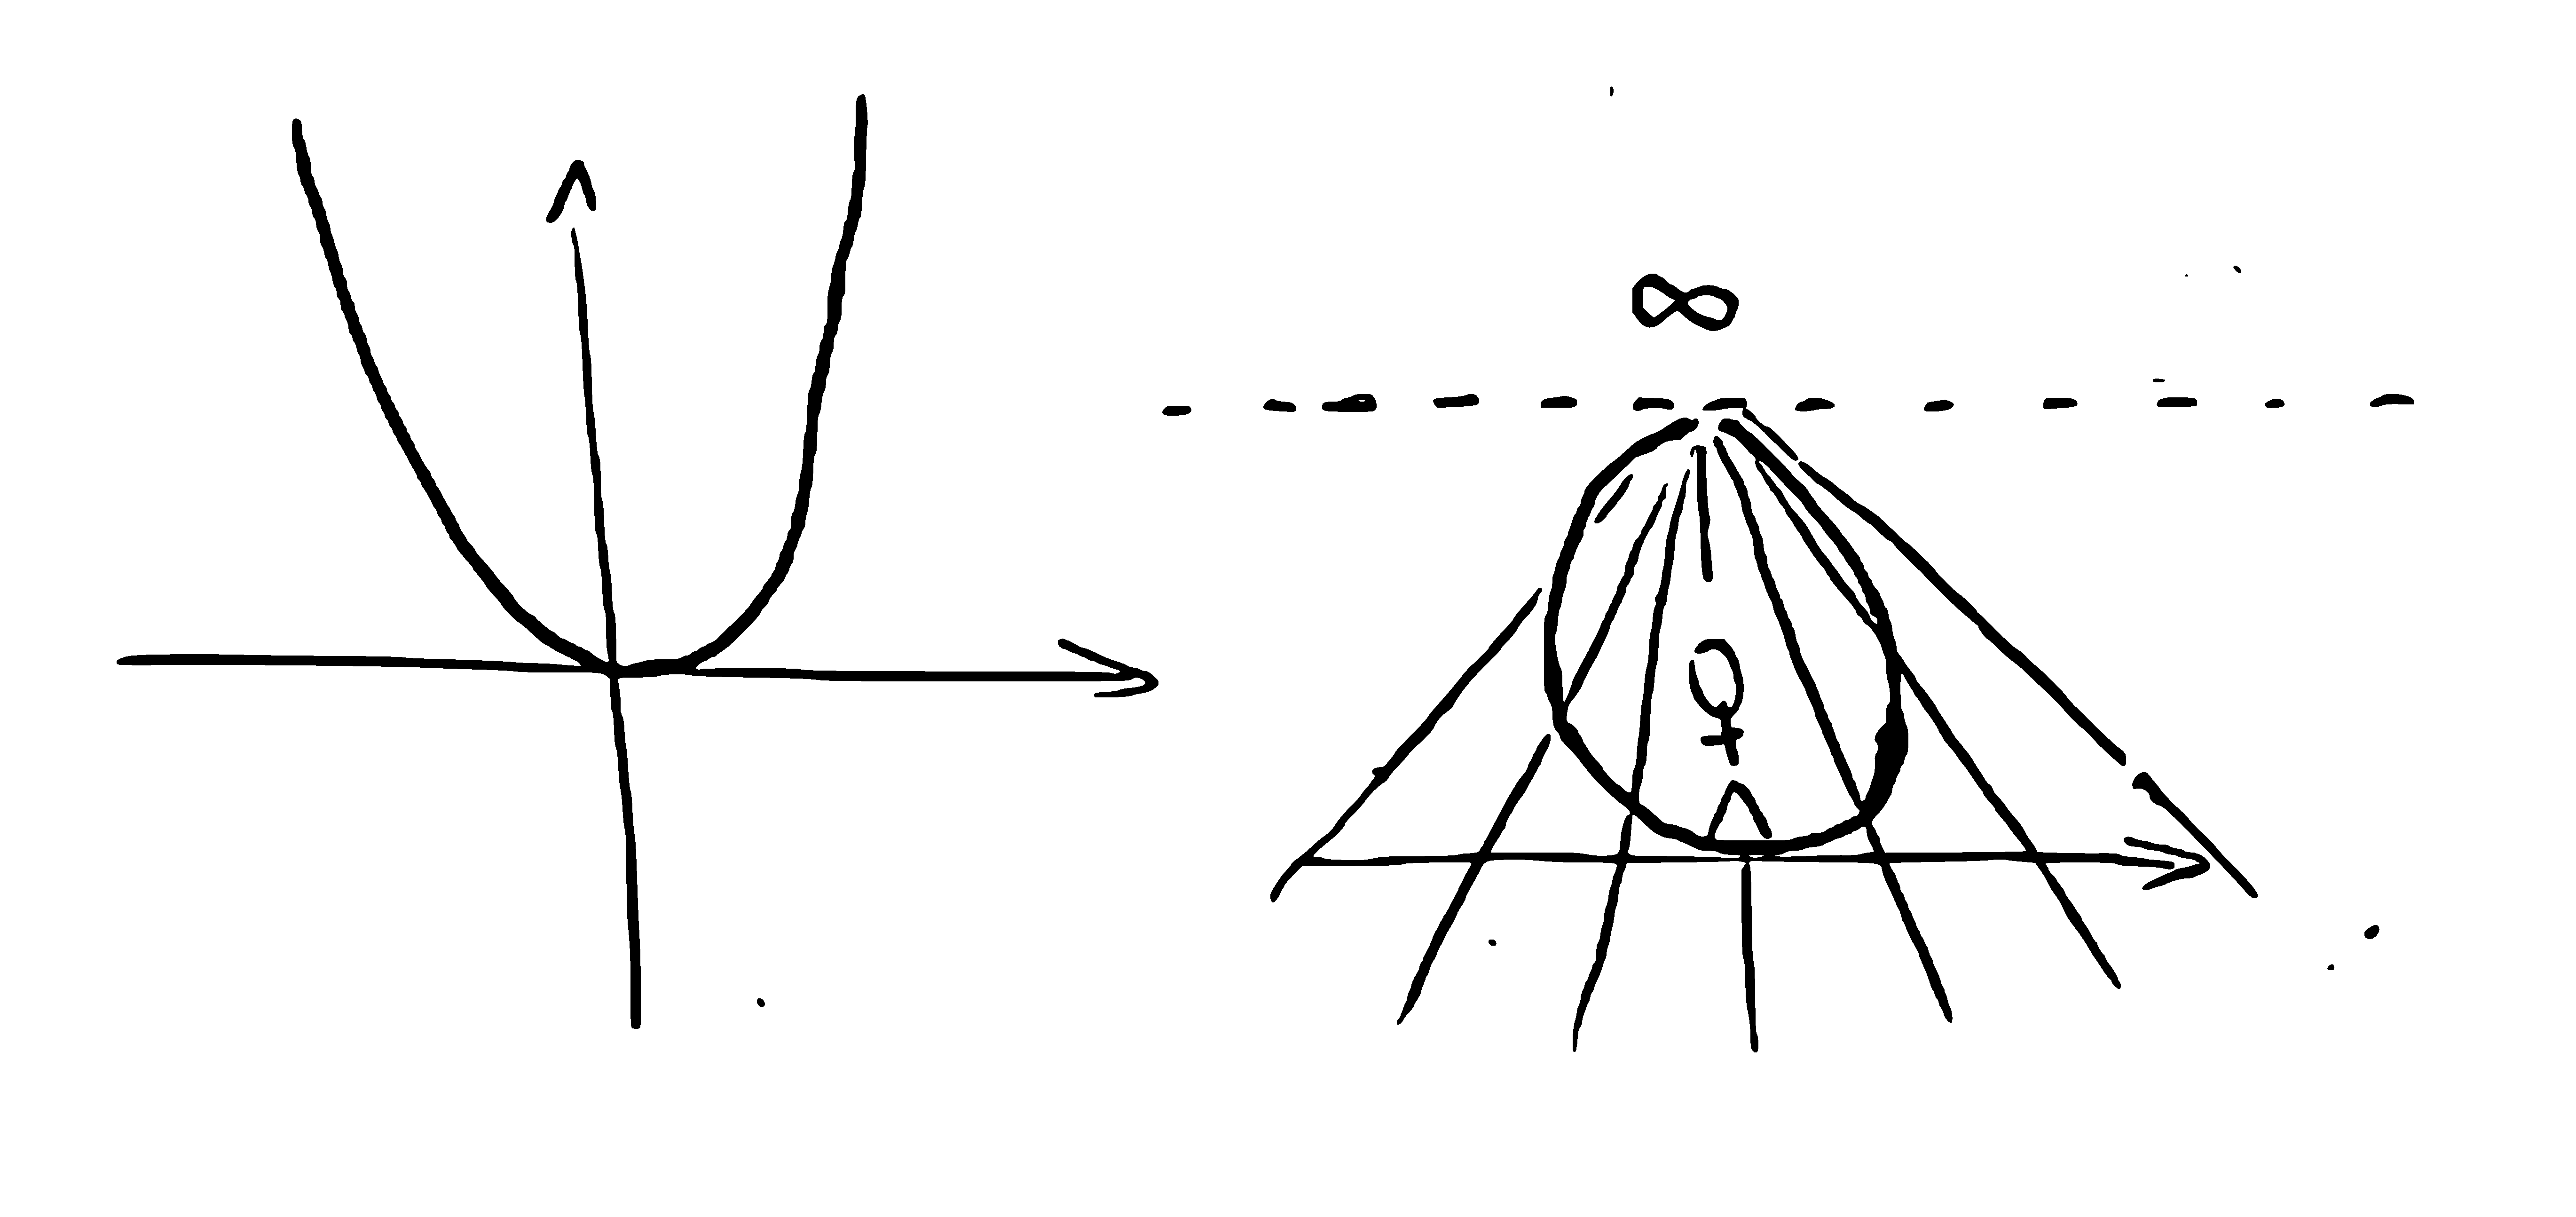
\includegraphics[width=0.8\textwidth]{figures/projektiivinen-paraabeli.pdf}
    \caption{Paraabeli $\R^2$:ssa ja $\P^2(\R)$:ssa, jossa se muistuttaa ellipsiä.}
    \label{kuva:projektiivinen-paraabeli}
\end{figure*}
Sulkeutuuko algebrallinen käyrä aina äärettömyydessä? Ei välttämättä. Kartioleikkauksista hyperboli antaa vastaesimerkin.

Annetuista esimerkeistä hyperboli on itse asiassa kiinnostavin, sillä se paljastaa jotakin oleellista projektiivisen avaruuden rakenteesta, nimittäin sen, että avaruutta ympäröivä horisontti ei ole yksinkertaisesti vain ympyrä. Tilannetta havainnollistetaan jokseenkin monimutkaisessa kuvassa~\ref{kuva:projektiivinen-hyperboli}.
\begin{figure*}
    \centering
    \includegraphics[width=0.7\textwidth]{figures/projektiivinen-hyperboli.pdf}
    \caption{Hyperboli $\R^2$:ssa ja $\P^2(\R)$:ssa.}
    \label{kuva:projektiivinen-hyperboli}
\end{figure*}
Kuvassa vasemmalla on esitetty hyperboli tutussa reaalitasossa. Kuvaan on lisäksi merkitty kaksi asymptoottisuoraa $h_1$ ja $h_2$, joita kohti hyperboli suppenee neljässä eri suunnassa.
\begin{esimerkki}[Projektiivinen hyperboli]
    Hyperbolin yhtälö on $f(x,y)=x^2-y^2+1=0$, jonka homogenisoitu muoto on $F(X,Y,Z)=X^2-Y^2+Z^2=0$. Horisontti vastaa pisteitä, joilla $Z=0$. Yhtälö äärettömyydessä on siis $X^2-Y^2=0$. Tällöin
    \begin{align*}
        X^2-Y^2 &= 0 \\
        (X-Y)(X+Y) &= 0,
    \end{align*}
    jolloin $X=\pm Y$. Tämä vastaa pisteitä $[X:Y:0]\sim[1:1:0]$ ja $[X:-Y:0]\sim[1:-1:0]$. Nämä pisteet vastaavat hyperbolin kahta asymptoottisuoraa $h_1$ ja $h_2$. $F$:n osittaisderivaatat ovat
    \begin{equation*}
        \frac{\partial F}{\partial X} = 2X,\quad
        \frac{\partial F}{\partial Y} = -2Y,\quad
        \frac{\partial F}{\partial Z} = 2Z.
    \end{equation*}
    Tangenttisuorat pisteissä $[1:1:0]$ ja $[1:-1:0]$ ovat siis $X-Y=0$ ja $X+Y=0$. Nämä vastaavat suoria $h_2$ ja $h_1$.
\end{esimerkki}
Oikealla on päällekkäin kaksi reaalista projektiivista tasoa. Keskitytään ensiksi alempaan tikku-ukkoon. Kuten edellisissä kuvissa, tikku-ukko seisoo origossa ja katsoo horisonttiin. Tämä vastaa vasemmanpuoleisen kuvan ylempää puolitasoa $y>0$. Hyperboli on piirretty tasaisella viivalla ja se törmää horisonttiin kahdessa pisteessä muodostaen ellipsin. Tikku-ukon avaruuden oikealla puolella on ympyrä, joka esittää positiivisen kiertosuunnan.

Mitä tapahtuu horisontin takana, johon on piirretty katkoviivaa? Siirrytään takaisin vasemmanpuoleiseen kuvaan $\R^2$:een. Oletetaan, että tikku-ukko lähtee kävelemään paraabelia pitkin luoteeseen ja että hän saapuu äärettömyyteen. Äärettömyydessä hänen pistettään vastaa asymptoottinen suora $h_1$, mutta hän olisi voinut kulkea myös kaakkoon päästäkseen tähän pisteeseen! Toisin sanoen kävelemällä eteenpäin äärettömyyteen ja sen yli, tikku-ukko päätyykin alapuoliseen tasoon ($y<0$). Jos hän jatkaa matkaa, hän saapuu ennen pitkää takaisin origoon.

Tikku-ukon matkalla avaruus on kuitenkin kääntynyt 180 astetta. Tätä havainnollistavat kuvan oikealla laidalla olevat kiertoympyrät, jotka kääntyvät 180 astetta avaruuden yli mentäessä. Jos origon tienoilta lähtisi armeija tikku-ukkoja ympyrämuodostelmassa kävelemään kohti äärettömyyttä, he päätyisivät ennen pitkää takaisin origoon, mutta heidän ympyränsä olisi nyt kääntynyt 180 astetta alkuperäisestä. Tämä johtuu siitä, että projektiivisessa avaruudessa luode vastaa kaakkoa ja koillinen lounasta. Tilanteen voi onneksi korjata kävelemällä uudestaan äärettömyyden yli.

Projektiivista tasoa ei siis ympäröikään ympyrä, vaan ympyrä jossa kaksi vastakkaista pistettä ovatkin sama piste. Kyseessä on siis puoliympyrä, mutta miten puoliympyrä voi ympyröidä avaruutta, jossa on kuitenkin ympyrän verran liikkumasuuntia? Jätämme tämän lukijan pohdittavaksi.